\documentclass[11pt]{beamer}
\usepackage[utf8]{inputenc}
\usepackage[T1]{fontenc}
\usepackage{lmodern}
\usepackage[italian]{babel}
\usepackage{tikz}
\usepackage{tabularx}
\usepackage{xparse}
\usetikzlibrary{automata,positioning}
\definecolor{mycolor}{RGB}{204,204,255}
\usetheme{Boadilla}

\makeatletter
\def\superclasses{}

\newcommand{\addsuperclasses}[1]{
	\def\superclasses{
		\multicolumn{2}{|>{\hsize=\dimexpr2\hsize+2\tabcolsep+\arrayrulewidth\relax}X|}{\scriptsize Superclasses}\\\hline
		\multicolumn{2}{|>{\hsize=\dimexpr2\hsize+2\tabcolsep+\arrayrulewidth\relax}X|}{\scriptsize #1}\\\hline
	}
}

\newenvironment{crccard}[3][]{
	\center
%	\table
	\tabularx{.9\textwidth}{ |*{2}{X|} }
%	\centering
	\superclasses
	\def\superclasses{}
	\hline
	\multicolumn{2}{|>{\hsize=\dimexpr2\hsize+2\tabcolsep+\arrayrulewidth\relax}X|}{\textbf{#2}}\\\hline
	\multicolumn{2}{|>{\hsize=\dimexpr2\hsize+2\tabcolsep+\arrayrulewidth\relax}X|}{\scriptsize #3}\\\hline
	\textbf{\scriptsize Responsabilità} & \textbf{\scriptsize Collaboratori}\\\hline
}{
	\endtabularx
	\endcenter
%	\endtable
}
\makeatother

\newcommand{\crcrow}[2][]{\scriptsize #2 & \scriptsize #1 \\\hline}


\begin{document}
	\author{Ciraolo, Porta, Rizzi}
	%\subtitle{}
	%\logo{}
	%\institute{}
	%\date{}
	%\subject{}
	%\setbeamercovered{transparent}
	%\setbeamertemplate{navigation symbols}{}

	\begin{frame}[plain]
		\title[IiNA System]{Seconda review\\IiNA System}
		\date{11 Gennaio 2022}
		\maketitle
	\end{frame}

	\begin{frame}
		\frametitle{Nuovo status Trello}
		\begin{figure}
			\centering
			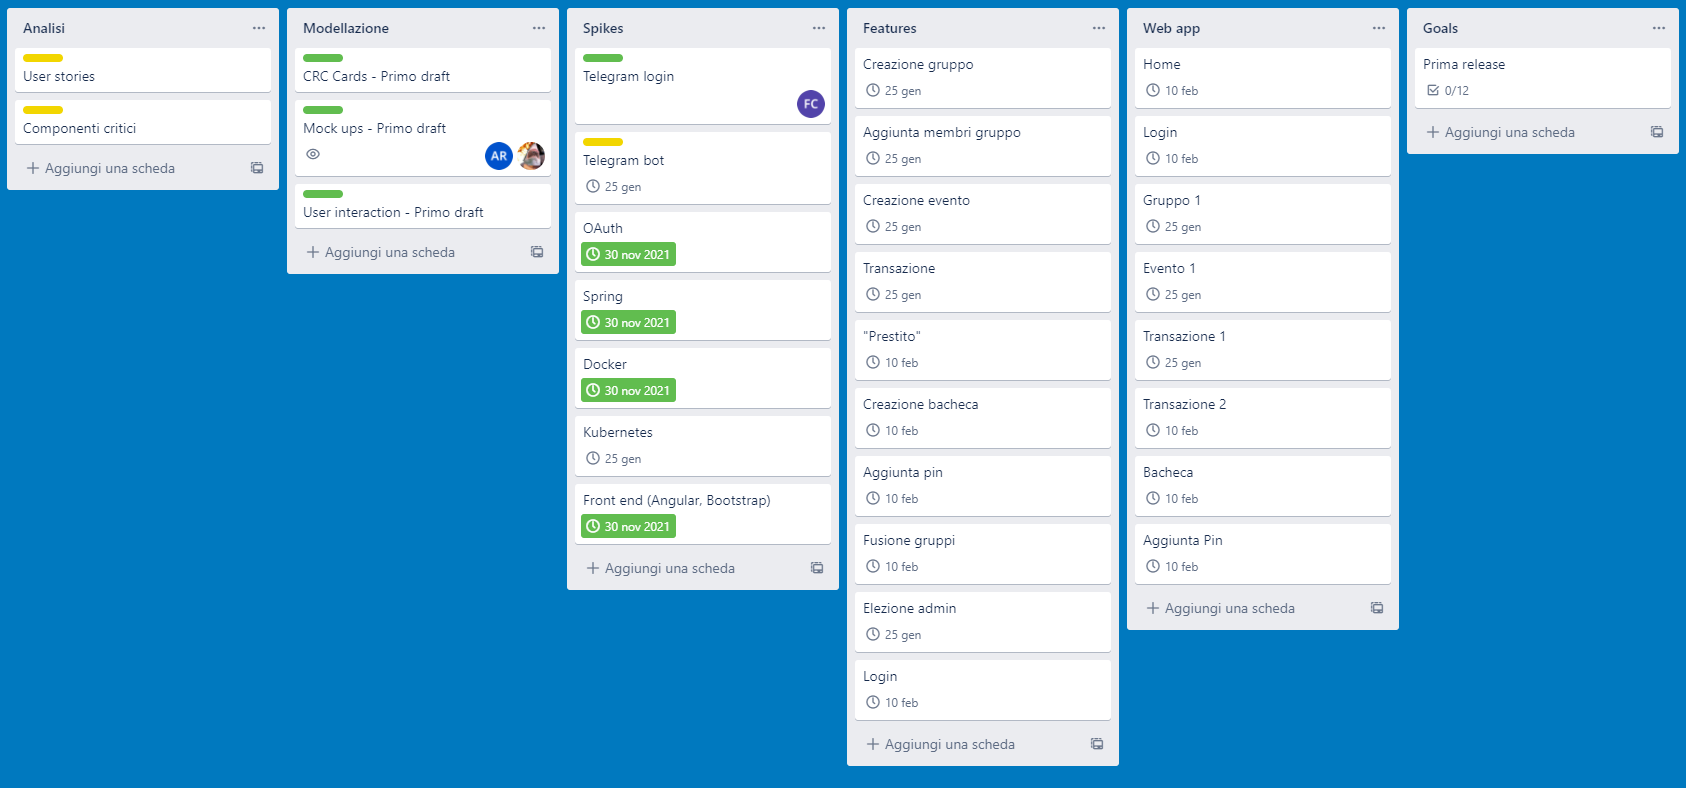
\includegraphics[width=\linewidth]{trello2}
		\end{figure}
	\end{frame}

	\begin{frame}
		\frametitle{Class Diagram}
		\begin{figure}
			\centering
			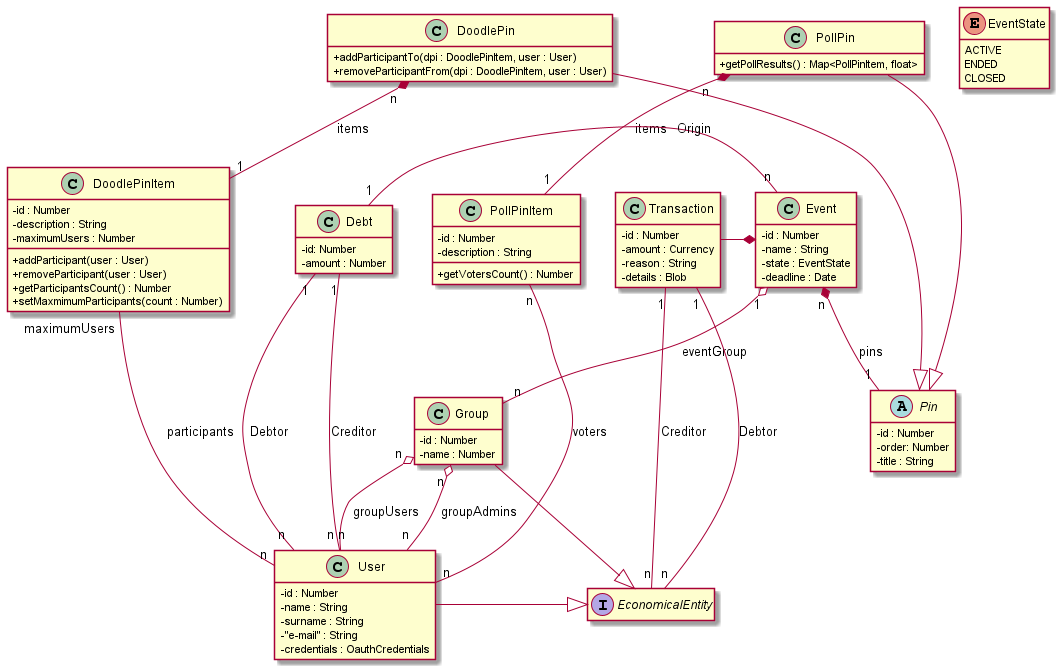
\includegraphics[width=\linewidth]{out/class_diagram/Class Diagram}
		\end{figure}
	\end{frame}	
	
	\begin{frame}
		\frametitle{Architettura (All'11 Gennaio)}
		\begin{figure}
			\centering
			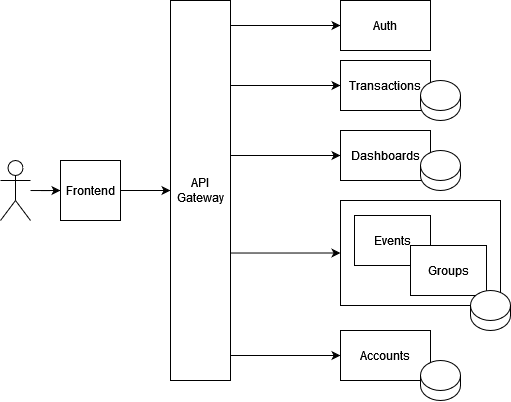
\includegraphics[width=0.8\linewidth]{Architecture Draft}
		\end{figure}
	\end{frame}

	\begin{frame}[plain]
		\begin{tikzpicture}[overlay, remember picture]
			\node[anchor=center] at (current page.center) {
				\begin{beamercolorbox}[center]{title}
					{\Huge Grazie per l'attenzione}\\
					\Large Domande?
			\end{beamercolorbox}};
		\end{tikzpicture}
	\end{frame}

	\begin{frame}[plain]
		\title[IiNA System]{Prima review\\IiNA System}
		\date{15 Novembre 2021}
		\maketitle
	\end{frame}
	
	\begin{frame}
		\frametitle{Project goals and NO goals}
		
		\begin{columns}
			\begin{column}{.45\linewidth}
				\begin{center}
					\textbf{Goals}
				\end{center}
				\begin{itemize}
					\item Semplificare la risoluzione di debiti e crediti in gruppi di fiducia
					\item Pianificazione e votazione di eventi o parte degli stessi
					\item Creazione di gruppi modulari con preferenze su creditori e debitori
					\item Integrazione bot con Telegram e altre app di messaggistica
				\end{itemize}
			\end{column}
			\begin{column}{.45\linewidth}
				\begin{center}
					\textbf{No Goals}
				\end{center}
				\begin{itemize}
					\item Non è un "portafogli" e non tiene valore economico
					\item Non gestisce i pagamenti fra gli utenti%\footnotemark[1]
					\item Non implementa un sistema per trovare partecipanti
				\end{itemize}
			\end{column}
		\end{columns}
%		\footnotetext[1]{Potenziale aggiunta futura}
	\end{frame}

	\begin{frame}
		\frametitle{Motivations}
		
		\begin{itemize}
			\item Comodità nella gestione dei gruppi
			\item Facilità di saldo di crediti e debiti data la risoluzione ottimizzata
			\item Mantenimento di \textit{prove di acquisto}
			\item Automatizzazione della risoluzione
			\item Planning del viaggio o degli eventi
			\item Decisioni condivise e democratiche
			\item Organizzazione di grandi gruppi, eventualmente modulari
			\item[] 
\includegraphics[width=.1\linewidth]{gnu.png}
		\end{itemize}
	\end{frame}

	\begin{frame}
		\frametitle{Similar applications}
		
		\begin{itemize}
			\item \href{https://play.google.com/store/apps/details?id=com.Splitwise.SplitwiseMobile&hl=en_US&gl=US}{Splitwise}
			\item \href{https://play.google.com/store/apps/details?id=com.tribab.tricount.android}{Tricount}
			\item \href{https://play.google.com/store/apps/details?id=org.marbot.travel.money.free}{Travel Money}
			\item \href{https://play.google.com/store/apps/details?id=com.jwang123.splitbills}{Split Bills}
		\end{itemize}
	\end{frame}

	\begin{frame}
		\frametitle{Initial Project plan summary}
		
		% TODO: \usepackage{graphicx} required
		\begin{figure}
			\centering
			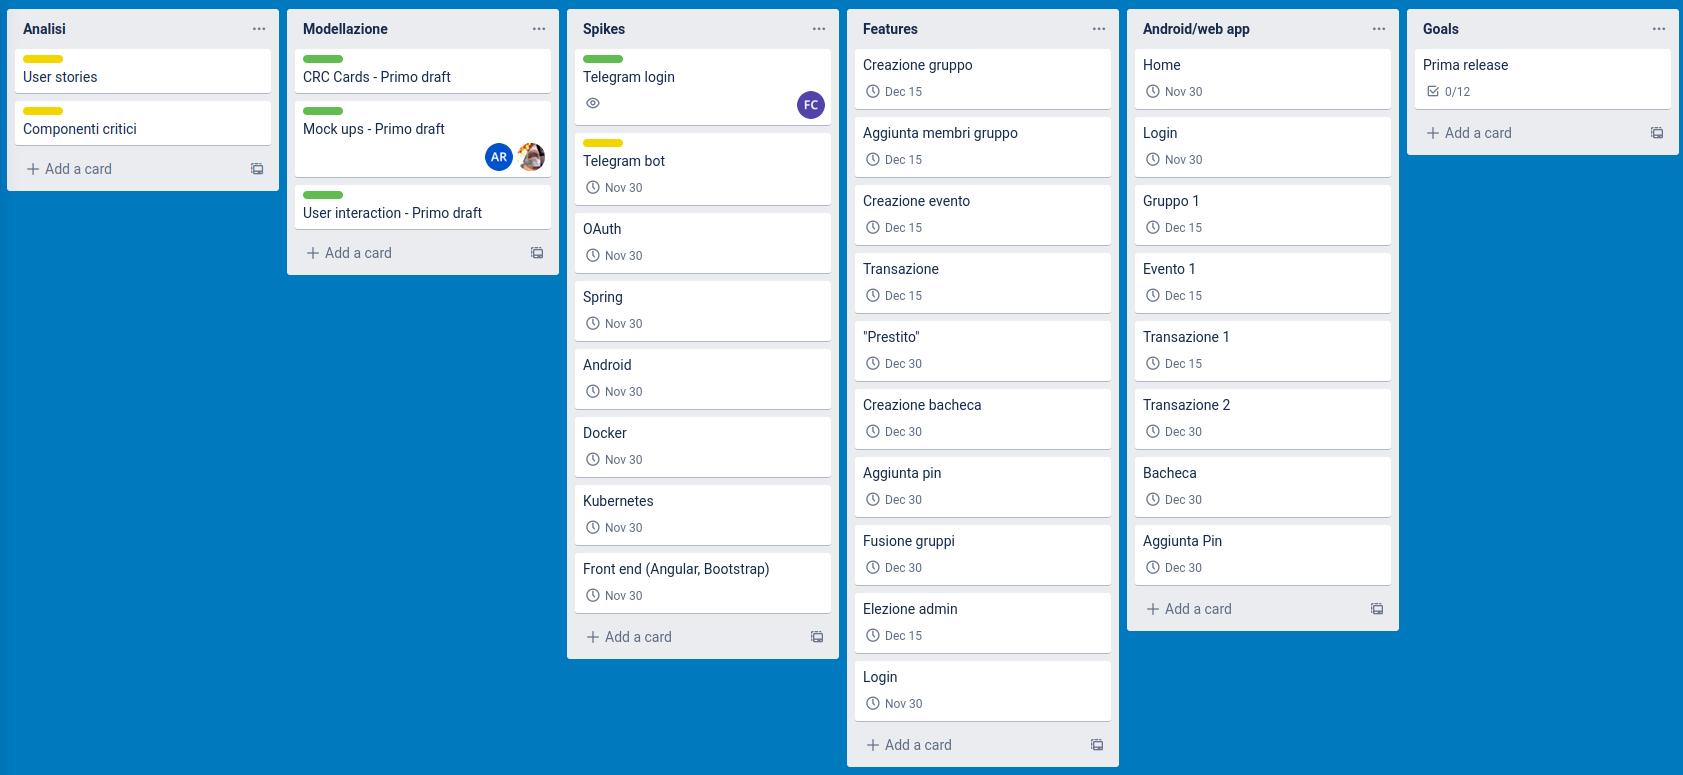
\includegraphics[width=\linewidth]{trello}
%			\caption{}
%			\label{fig:trello}
		\end{figure}
		
%		% TODO: telegram bot development
%		\begin{columns}
%			\begin{column}{.45\linewidth}
%				\begin{itemize}
%					\item Novembre
%					\begin{itemize}
%						\item Spikes
%						\item Analisi componenti critici 
%						\item Modellazione delle funzionalità principali
%						\item Mockups dettagliati
%						\item Sviluppo iniziale del core
%					\end{itemize}
%					\item 15/12/21
%					\begin{itemize}
%						\item Gestione dei gruppi a livello singolo
%						\item Elezioni admin
%						\item Primi stadi web app e android app
%					\end{itemize}
%				\end{itemize}
%			\end{column}
%			\begin{column}{.45\linewidth}
%				\begin{itemize}
%					\item Fine Dicembre
%					\begin{itemize}
%						\item Gruppi multilivello
%						\item Debiti individuali
%						\item Board
%						\item Secondo stadio delle applicazioni
%					\end{itemize}
%					\item Metà gennaio
%					\begin{itemize}
%						\item Pools e planning
%						\item Refactoring and polishing
%						\item Completamento prima release applicazioni
%					\end{itemize}
%				\end{itemize}
%			\end{column}
%		\end{columns}
		
%		\begin{itemize}
%			\item Novembre
%			\begin{itemize}
%				\item Spikes
%				\item Analisi componenti critici 
%				\item Modellazione delle funzionalità principali
%				\item Mockups dettagliati
%				\item Sviluppo iniziale del core
%			\end{itemize}
%			\item 15/12/21
%			\begin{itemize}
%				\item Gestione dei gruppi a livello singolo
%				\item Elezioni admin
%				\item Primi stadi web app e android app
%			\end{itemize}
%			\item Fine Dicembre
%			\begin{itemize}
%				\item Gruppi multilivello
%				\item Debiti individuali
%				\item Board
%				\item Secondo stadio delle applicazioni
%			\end{itemize}
%			\item Metà gennaio
%			\begin{itemize}
%				\item Pools e planning
%				\item Refactoring and polishing
%				\item Completamento prima release applicazioni
%			\end{itemize}
%		\end{itemize}
	\end{frame}

	\begin{frame}
		\frametitle{Status as of November 15, 2021}
		
		\begin{itemize}
			\item User stories
			\item Alcuni spikes
			\item Mockups
			\item Bozza di interazioni
			\item CRC cards
		\end{itemize}
	\end{frame}

	\section{User stories}
	
	\begin{frame}
		\begin{itemize}
			\item \textbf{Creazione del gruppo}
			
			\item[] Stiamo partendo in vacanza noi 10 del gruppo e abbiamo deciso di gestire le spese per ridurre al minimo il giro di piccoli pagamenti fra noi.
			
			Creiamo un gruppo in cui aggiungiamo tutti i partecipanti alla gita e poniamo un budget per la vacanza come indicatore.
			
			\item \textbf{Aggiunta costo sostenuto}
			
			\item[] Mentre stiamo andando verso il Monte Bianco iniziamo a pagare il primo pedaggio, siamo divisi in tre auto e il costo è fisso per tutte.
			
			Subito dopo aver pagato aggiungiamo i tre costi sostenuti al sistema con una descrizione degli stessi. Viene aggiunta la data e posso allegare la foto della ricevuta.
		\end{itemize}
	\end{frame}

	\begin{frame}
		\begin{itemize}
			\item \textbf{Aggiunta credito uno a uno}
			
			\item[] Mario ha pagato i 18 euro di pedaggio ma gli mancavano le monete e gliele ho fornite io, per cui ho aggiunto al sistema questo credito verso Mario; alla risoluzione ne verrà tenuto in conto.
			
			Serve solo che lui confermi questa transazione per aggiungerla allo storico.
			
			\item \textbf{Risoluzione dei debiti}
			
			\item[] La vacanza è finita e vanno saldati i conti, chiudiamo il gruppo ed il sistema risolve i debiti in modo da avere la lista finale di debiti ottimizzata. Ovvero con ciascuno solo debitore o creditore e un numero di transazioni ridotte al minimo.
		\end{itemize}
	\end{frame}

	\begin{frame}
		\begin{itemize}
			\item \textbf{Votazioni e organizzazione}
			
			\item[] Nel prepare la scampagnata dobbiamo decidere cosa portare in tavola. Siamo in tanti e l'organizzazione risulta complicata.
			
			Creo il gruppo come amministratore e apro una bacheca; in essa ciascuno può inserire se si impegna a portare qualcosa ed in seguito aggiungerà il costo sostenuto.
			
			Prima però dobbiamo decidere tutti insieme cosa mangiare per cui creo dei sondaggi sulle varie portate e ciascuno può esprimere la preferenza.
			
			\item \textbf{Amministrazione}
			
			\item[] Deciso il cibo mi rendo conto che non ho spazio a sufficienza in casa per tenere anche le bevande per cui chiedo a qualcun altro di amministare la gestione delle bibite.
			
			Possiamo tutti votare per un nuovo admin, che si sia candidato, e chi prende più voti diventa il nostro \textit{sommelier}.
		\end{itemize}
	\end{frame}

	\begin{frame}
		\begin{itemize}
			\item \textbf{Fusione di gruppi}
			
			\item[] Lucia si laurea la prossima settimana e noi del gruppo dell'Università abbiamo deciso di fare un regalo insieme; nel frattempo però il suo gruppo di amici da casa ci ha contattato proponendo di fare un regalo più grande insieme.
			
			A questo punto abbiamo deciso di unire il nostro gruppo regalo già fatto al loro e provare ad organizzare il regalo, sia nella decisione che nella raccolta dei fondi, tutti insieme.
			
			Nell'unire i due gruppi vengono considerati i partecipanti in modo che il costo sia diviso equamente ad eccezione di chi vuol contribuire di più per i fatti loro.
			
			Gli amministratori dei due gruppi, se assenti vengono eletti, diventano i responsabili per il proprio gruppo e fra loro avviene, se possibile, il saldo economico fra i due gruppi.
			
			Le votazioni sono come sempre e ciascuno ha un voto unitario.
		\end{itemize}
	\end{frame}
	
	\begin{frame}
		\frametitle{Spikes to be done}
		
		\begin{itemize}
			\item Spring
			\item Android
			\item Frontend da definire
			\item Docker
			\item Kubernetes
			\item OAuth
			\item Telegram bot
		\end{itemize}
	\end{frame}
	
	\begin{frame}
		\frametitle{User Interaction Draft}
		\tikzset{app state/.style={fill=blue!20, draw,minimum size=1.5cm,inner sep=0pt,text width=1.5cm, align=center}}
		
		\tiny
		
		\begin{figure}
			\begin{tikzpicture}

				\node[state, minimum size=1.2cm,fill=mycolor] (event) {Evento};
				\node[state, minimum size=1.2cm,fill=mycolor] (group) [below = 2cm of event] {Gruppo};
				\node[state, minimum size=1.2cm,fill=mycolor] (home) [below left = 0.5cm and 2.5cm of event] {Home};
				\node[state, minimum size=1.2cm,fill=mycolor] (report) [above = 1.5cm of home] {Report};
				\node[state, minimum size=1.2cm,fill=mycolor] (pin) [above = 1.6cm of event] {Pin};
				\node[state, minimum size=1.2cm,fill=mycolor] (transazione) [below right = 0.5cm and 2.5cm of event] {Transazione};
				\node[state, minimum size=1.2cm,fill=mycolor] (bacheca) [above = 1.5cm of transazione] {Bacheca};
				
				\draw[->] (home) edge node[above,sloped] {Apri evento} (event);
				\draw[->] (home) edge node[below,sloped] {Crea evento} (event);
				
				\path[->] (event) edge node[below,sloped] {Chiudi evento} (report);
				
				\path[->] (home) edge node[above,sloped] {Apri report} (report);
				
				\path[->] (event) edge node[above,sloped] {Apri bacheca} (bacheca);
				\path[->] (event) edge node[below,sloped] {Aggiungi pin} (bacheca);
				
				\path[->] (home) edge node[above,sloped] {Apri gruppo} (group);
				\path[->] (home) edge node[below,sloped] {Crea gruppo} (group);
				
				\path[->] (event) edge node[below,sloped] {Lista partecipanti} (group);
				\path[->] (group) edge node[below,sloped] {Lista eventi} (event);
				
				\path[->] (bacheca) edge node[above,sloped] {Crea pin} (pin);
				\path[->] (event) edge node[above,sloped] {Pin attivi} (pin);
				\path[->] (bacheca) edge node[below,sloped] {Interegisci pin} (pin);
				
				\path[->] (event) edge node[above,sloped] {Aggiungere transazione} (transazione);
				\path[->] (event) edge node[below,sloped] {Visualizzare transazione} (transazione);
				
				\path[->] (group) edge[loop right = 0.5cm] node{{Aggiungi partecipante}, {Rimuovi partecipante}}(group);
				
				
			\end{tikzpicture}
		\end{figure}
	\end{frame}

	\section{}
	
%	\begin{frame}
%		\begin{itemize}
%			\item Utente
%			\item Amministratore
%			\item Gruppo {stato}
%			\item Evento {budget}
%			\item Ente economica -> {Utente, Gruppo}
%			\item Transazione {creditore, debitore, importo, dettagli}
%			\item Debito {creditore, debitore, importo}
%			\item Bacheca
%			\item Pin
%			\item 
%		\end{itemize}
%	\end{frame}
	
	\begin{frame}
		\frametitle{CRC Cards – First draft - 1/6}
		
		\begin{table}
			\begin{tabularx}{.9\textwidth}{ |*{2}{X|} }
				\hline
				\multicolumn{2}{|>{\hsize=\dimexpr2\hsize+2\tabcolsep+\arrayrulewidth\relax}X|}{\textbf{Ente economico}}\\\hline
				\multicolumn{2}{|>{\hsize=\dimexpr2\hsize+2\tabcolsep+\arrayrulewidth\relax}X|}{\textit{Descrizione}: \scriptsize Interfaccia per modellare generico creditore o debitore, sia esso individuo o gruppo}\\\hline
			\end{tabularx}
		\end{table}
		
		\begin{table}
			\begin{tabularx}{.9\textwidth}{ |*{2}{X|} }
				\hline
				\multicolumn{2}{|>{\hsize=\dimexpr2\hsize+2\tabcolsep+\arrayrulewidth\relax}X|}{\textbf{Utente}}\\\hline
				\multicolumn{2}{|>{\hsize=\dimexpr2\hsize+2\tabcolsep+\arrayrulewidth\relax}X|}{\textit{Superclassi}: \scriptsize Ente economico}\\\hline
				\multicolumn{2}{|>{\hsize=\dimexpr2\hsize+2\tabcolsep+\arrayrulewidth\relax}X|}{\textit{Descrizione}: \scriptsize Modella un generico utilizzatore del sistema}\\\hline
				\multicolumn{2}{|>{\hsize=\dimexpr2\hsize+2\tabcolsep+\arrayrulewidth\relax}X|}{\scriptsize \textbf{Attributi}}\\\hline
				\scriptsize \textit{Attributo} & \scriptsize \textit{Descrizione}\\\hline
				\scriptsize Anagrafica & \scriptsize I dati dell'utente\\\hline
			\end{tabularx}
		\end{table}
	\end{frame}

	\begin{frame}
		\frametitle{CRC Cards – First draft - 2/6}
		
		\begin{table}
			\begin{tabularx}{.9\textwidth}{ |*{2}{X|} }
				\hline
				\multicolumn{2}{|>{\hsize=\dimexpr2\hsize+2\tabcolsep+\arrayrulewidth\relax}X|}{\textbf{Gruppo}}\\\hline
				\multicolumn{2}{|>{\hsize=\dimexpr2\hsize+2\tabcolsep+\arrayrulewidth\relax}X|}{\textit{Superclassi}: \scriptsize Ente economico}\\\hline
				\multicolumn{2}{|>{\hsize=\dimexpr2\hsize+2\tabcolsep+\arrayrulewidth\relax}X|}{\textit{Descrizione}: \scriptsize Modella un gruppo di utenti che condividono spese e decidono per un evento}\\\hline
				\multicolumn{2}{|>{\hsize=\dimexpr2\hsize+2\tabcolsep+\arrayrulewidth\relax}X|}{\scriptsize \textbf{Responsabilità}}\\\hline
				\scriptsize \textit{Responsabilità} & \scriptsize \textit{Collaboratori}\\\hline
				\scriptsize Mantenere un insieme di utenti e gruppi di utenti & \scriptsize Utente, Gruppo\\\hline
				\scriptsize Mantenere l'insieme degli utenti con priviligi di amministrazione & \scriptsize Utente\\\hline
			\end{tabularx}
		\end{table}
	\end{frame}

	\begin{frame}
		\frametitle{CRC Cards – First draft - 3/6}
		
		\begin{table}
			\begin{tabularx}{.9\textwidth}{ |*{2}{X|} }
				\hline
				\multicolumn{2}{|>{\hsize=\dimexpr2\hsize+2\tabcolsep+\arrayrulewidth\relax}X|}{\textbf{Evento}}\\\hline
%				\multicolumn{2}{|>{\hsize=\dimexpr2\hsize+2\tabcolsep+\arrayrulewidth\relax}X|}{\textit{Superclassi}: \scriptsize Ente economico}\\\hline
				\multicolumn{2}{|>{\hsize=\dimexpr2\hsize+2\tabcolsep+\arrayrulewidth\relax}X|}{\textit{Descrizione}: \scriptsize Evento (presente o pianificato) a cui partecipa (o parteciperà) un gruppo di utenti}\\\hline
				\multicolumn{2}{|>{\hsize=\dimexpr2\hsize+2\tabcolsep+\arrayrulewidth\relax}X|}{\scriptsize \textbf{Attributi}}\\\hline
				\scriptsize \textit{Attributo} & \scriptsize \textit{Descrizione}\\\hline
				\scriptsize Stato & \scriptsize Uno fra \{in corso, chiuso, ...\}\\\hline
				\scriptsize Budget & \scriptsize Opzionale soglia massima di riferimento per le spese\\\hline
				\scriptsize Deadline & \scriptsize Opzionale data limite per planning e acquisti\\\hline
				\multicolumn{2}{|>{\hsize=\dimexpr2\hsize+2\tabcolsep+\arrayrulewidth\relax}X|}{\scriptsize \textbf{Responsabilità}}\\\hline
				\scriptsize \textit{Responsabilità} & \scriptsize \textit{Collaboratori}\\\hline
				\scriptsize Mantenere il gruppo di partecipanti & \scriptsize Gruppo\\\hline
				\scriptsize Mantenere una lista delle transazioni & \scriptsize Transazione\\\hline
				\scriptsize Collegare ad un eventuale bacheca & \scriptsize Bacheca\\\hline
			\end{tabularx}
		\end{table}
	\end{frame}

	\begin{frame}
		\frametitle{CRC Cards – First draft - 4/6}
		
		\begin{table}
			\begin{tabularx}{.9\textwidth}{ |*{2}{X|} }
				\hline
				\multicolumn{2}{|>{\hsize=\dimexpr2\hsize+2\tabcolsep+\arrayrulewidth\relax}X|}{\textbf{Transazione}}\\\hline
				%				\multicolumn{2}{|>{\hsize=\dimexpr2\hsize+2\tabcolsep+\arrayrulewidth\relax}X|}{\textit{Superclassi}: \scriptsize Ente economico}\\\hline
				\multicolumn{2}{|>{\hsize=\dimexpr2\hsize+2\tabcolsep+\arrayrulewidth\relax}X|}{\textit{Descrizione}: \scriptsize Una transazione fra un creditore ed un debitore, con eventuali dettagli}\\\hline
				\multicolumn{2}{|>{\hsize=\dimexpr2\hsize+2\tabcolsep+\arrayrulewidth\relax}X|}{\scriptsize \textbf{Attributi}}\\\hline
				\scriptsize \textit{Attributo} & \scriptsize \textit{Descrizione}\\\hline
				\scriptsize Importo & \scriptsize Valore economico della transazione\\\hline
				\scriptsize Dettagli & \scriptsize Eventuali altre informazioni sulla transazione (immagini, date, ...)\\\hline
				\scriptsize Conferma & \scriptsize Eventuale conferma in caso di prestito\\\hline
				\multicolumn{2}{|>{\hsize=\dimexpr2\hsize+2\tabcolsep+\arrayrulewidth\relax}X|}{\scriptsize \textbf{Responsabilità}}\\\hline
				\scriptsize \textit{Responsabilità} & \scriptsize \textit{Collaboratori}\\\hline
				\scriptsize Mantenere traccia del debitore e del creditore & \scriptsize Ente economico\\\hline
%				\scriptsize Mantenere una lista delle transazioni & \scriptsize Transazione\\\hline
%				\scriptsize Collegare ad un eventuale bacheca & \scriptsize Bacheca\\\hline
			\end{tabularx}
		\end{table}
	\end{frame}

	\begin{frame}
		\frametitle{CRC Cards – First draft - 5/6}
		
		\begin{table}
			\begin{tabularx}{.9\textwidth}{ |*{2}{X|} }
				\hline
				\multicolumn{2}{|>{\hsize=\dimexpr2\hsize+2\tabcolsep+\arrayrulewidth\relax}X|}{\textbf{Debito}}\\\hline
				%				\multicolumn{2}{|>{\hsize=\dimexpr2\hsize+2\tabcolsep+\arrayrulewidth\relax}X|}{\textit{Superclassi}: \scriptsize Ente economico}\\\hline
				\multicolumn{2}{|>{\hsize=\dimexpr2\hsize+2\tabcolsep+\arrayrulewidth\relax}X|}{\textit{Descrizione}: \scriptsize Debito finale, proposto dal solver, fra utenti}\\\hline
				\multicolumn{2}{|>{\hsize=\dimexpr2\hsize+2\tabcolsep+\arrayrulewidth\relax}X|}{\scriptsize \textbf{Attributi}}\\\hline
				\scriptsize \textit{Attributo} & \scriptsize \textit{Descrizione}\\\hline
				\scriptsize Importo & \scriptsize Valore economico della transazione\\\hline
				%				\scriptsize Dettagli & \scriptsize Eventuali altre informazioni sulla transazione (immagini, date, ...)\\\hline
				%				\scriptsize Conferma & \scriptsize Eventuale conferma in caso di prestito\\\hline
				\multicolumn{2}{|>{\hsize=\dimexpr2\hsize+2\tabcolsep+\arrayrulewidth\relax}X|}{\scriptsize \textbf{Responsabilità}}\\\hline
				\scriptsize \textit{Responsabilità} & \scriptsize \textit{Collaboratori}\\\hline
				\scriptsize Mantenere traccia del debitore e del creditore & \scriptsize Utente\\\hline
				%				\scriptsize Mantenere una lista delle transazioni & \scriptsize Transazione\\\hline
				%				\scriptsize Collegare ad un eventuale bacheca & \scriptsize Bacheca\\\hline
			\end{tabularx}
		\end{table}
	\end{frame}

	\begin{frame}
		\frametitle{CRC Cards – First draft - 6/6}
		
		\begin{table}
			\begin{tabularx}{.9\textwidth}{ |*{2}{X|} }
				\hline
				\multicolumn{2}{|>{\hsize=\dimexpr2\hsize+2\tabcolsep+\arrayrulewidth\relax}X|}{\textbf{Bacheca}}\\\hline
				%				\multicolumn{2}{|>{\hsize=\dimexpr2\hsize+2\tabcolsep+\arrayrulewidth\relax}X|}{\textit{Superclassi}: \scriptsize Ente economico}\\\hline
				\multicolumn{2}{|>{\hsize=\dimexpr2\hsize+2\tabcolsep+\arrayrulewidth\relax}X|}{\textit{Descrizione}: \scriptsize Aggregatore ed organizer di pin di un evento}\\\hline
				%				\multicolumn{2}{|>{\hsize=\dimexpr2\hsize+2\tabcolsep+\arrayrulewidth\relax}X|}{\scriptsize \textbf{Attributi}}\\\hline
				%				\scriptsize \textit{Attributo} & \scriptsize \textit{Descrizione}\\\hline
				%				\scriptsize Stato & \scriptsize Uno fra \{in corso, chiuso, ...\}\\\hline
				%				\scriptsize Budget & \scriptsize Opzionale soglia massima di riferimento per le spese\\\hline
				%				\scriptsize Deadline & \scriptsize Opzionale data limite per planning e acquisti\\\hline
				\multicolumn{2}{|>{\hsize=\dimexpr2\hsize+2\tabcolsep+\arrayrulewidth\relax}X|}{\scriptsize \textbf{Responsabilità}}\\\hline
				\scriptsize \textit{Responsabilità} & \scriptsize \textit{Collaboratori}\\\hline
				\scriptsize Mantenere una collezione, ordinata dagli user, di pin & \scriptsize Pin\\\hline
				%				\scriptsize Mantenere una lista delle transazioni & \scriptsize Transazione\\\hline
				%				\scriptsize Collegare ad un eventuale bacheca & \scriptsize Bacheca\\\hline
			\end{tabularx}
		\end{table}
		
		\begin{table}
			\begin{tabularx}{.9\textwidth}{ |*{2}{X|} }
				\hline
				\multicolumn{2}{|>{\hsize=\dimexpr2\hsize+2\tabcolsep+\arrayrulewidth\relax}X|}{\textbf{Pin}}\\\hline
				%				\multicolumn{2}{|>{\hsize=\dimexpr2\hsize+2\tabcolsep+\arrayrulewidth\relax}X|}{\textit{Superclassi}: \scriptsize Ente economico}\\\hline
				\multicolumn{2}{|>{\hsize=\dimexpr2\hsize+2\tabcolsep+\arrayrulewidth\relax}X|}{\textit{Descrizione}: \scriptsize Interfaccia di vari "widget" ad uso degli utenti per organizzare un evento (sondaggi, calendari, note)}\\\hline
				%				\multicolumn{2}{|>{\hsize=\dimexpr2\hsize+2\tabcolsep+\arrayrulewidth\relax}X|}{\scriptsize \textbf{Attributi}}\\\hline
				%				\scriptsize \textit{Attributo} & \scriptsize \textit{Descrizione}\\\hline
				%				\scriptsize Stato & \scriptsize Uno fra \{in corso, chiuso, ...\}\\\hline
				%				\scriptsize Budget & \scriptsize Opzionale soglia massima di riferimento per le spese\\\hline
				%				\scriptsize Deadline & \scriptsize Opzionale data limite per planning e acquisti\\\hline
				%				\multicolumn{2}{|>{\hsize=\dimexpr2\hsize+2\tabcolsep+\arrayrulewidth\relax}X|}{\scriptsize \textbf{Responsabilità}}\\\hline
				%				\scriptsize \textit{Responsabilità} & \scriptsize \textit{Collaboratori}\\\hline
				%				\scriptsize Mantenere una collezione, ordinata dagli user, di pin & \scriptsize Pin\\\hline
				%				\scriptsize Mantenere una lista delle transazioni & \scriptsize Transazione\\\hline
				%				\scriptsize Collegare ad un eventuale bacheca & \scriptsize Bacheca\\\hline
			\end{tabularx}
		\end{table}
	\end{frame}
	
	\begin{frame}
		\frametitle{Mockups 1/2}
		\begin{figure}[h]
			\centering
			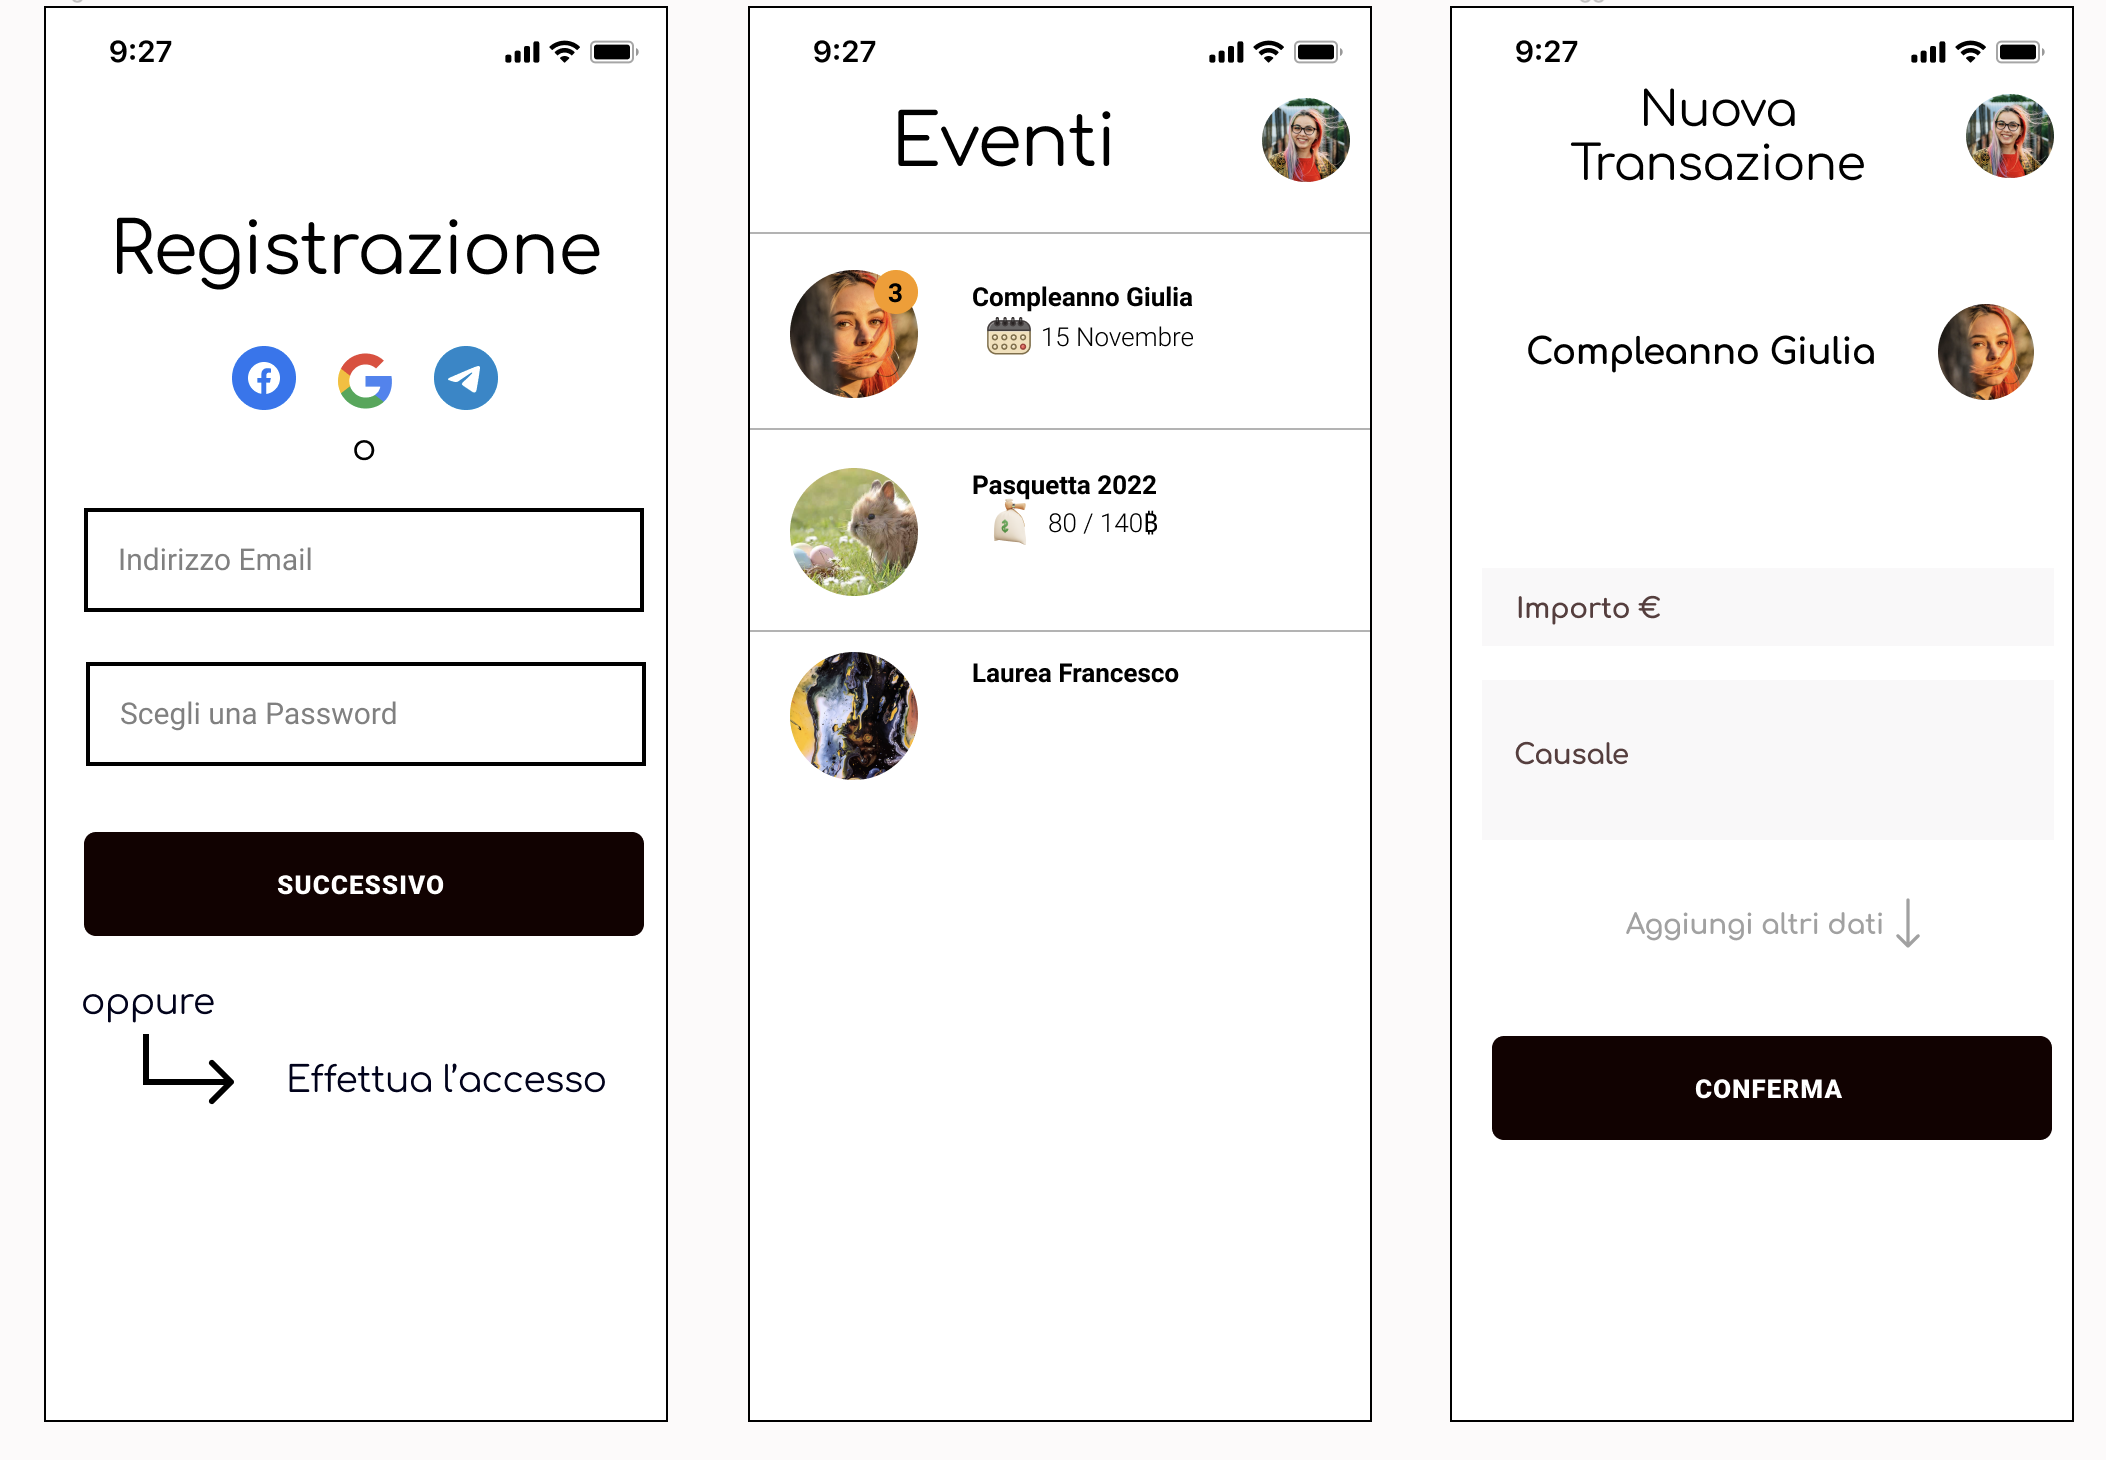
\includegraphics[width=.8\linewidth]{mock.png}
%			\caption{Mockups}
		\end{figure}
	\end{frame}

	\begin{frame}
		\frametitle{Mockups 2/2}
		\begin{figure}[h]
			\centering
			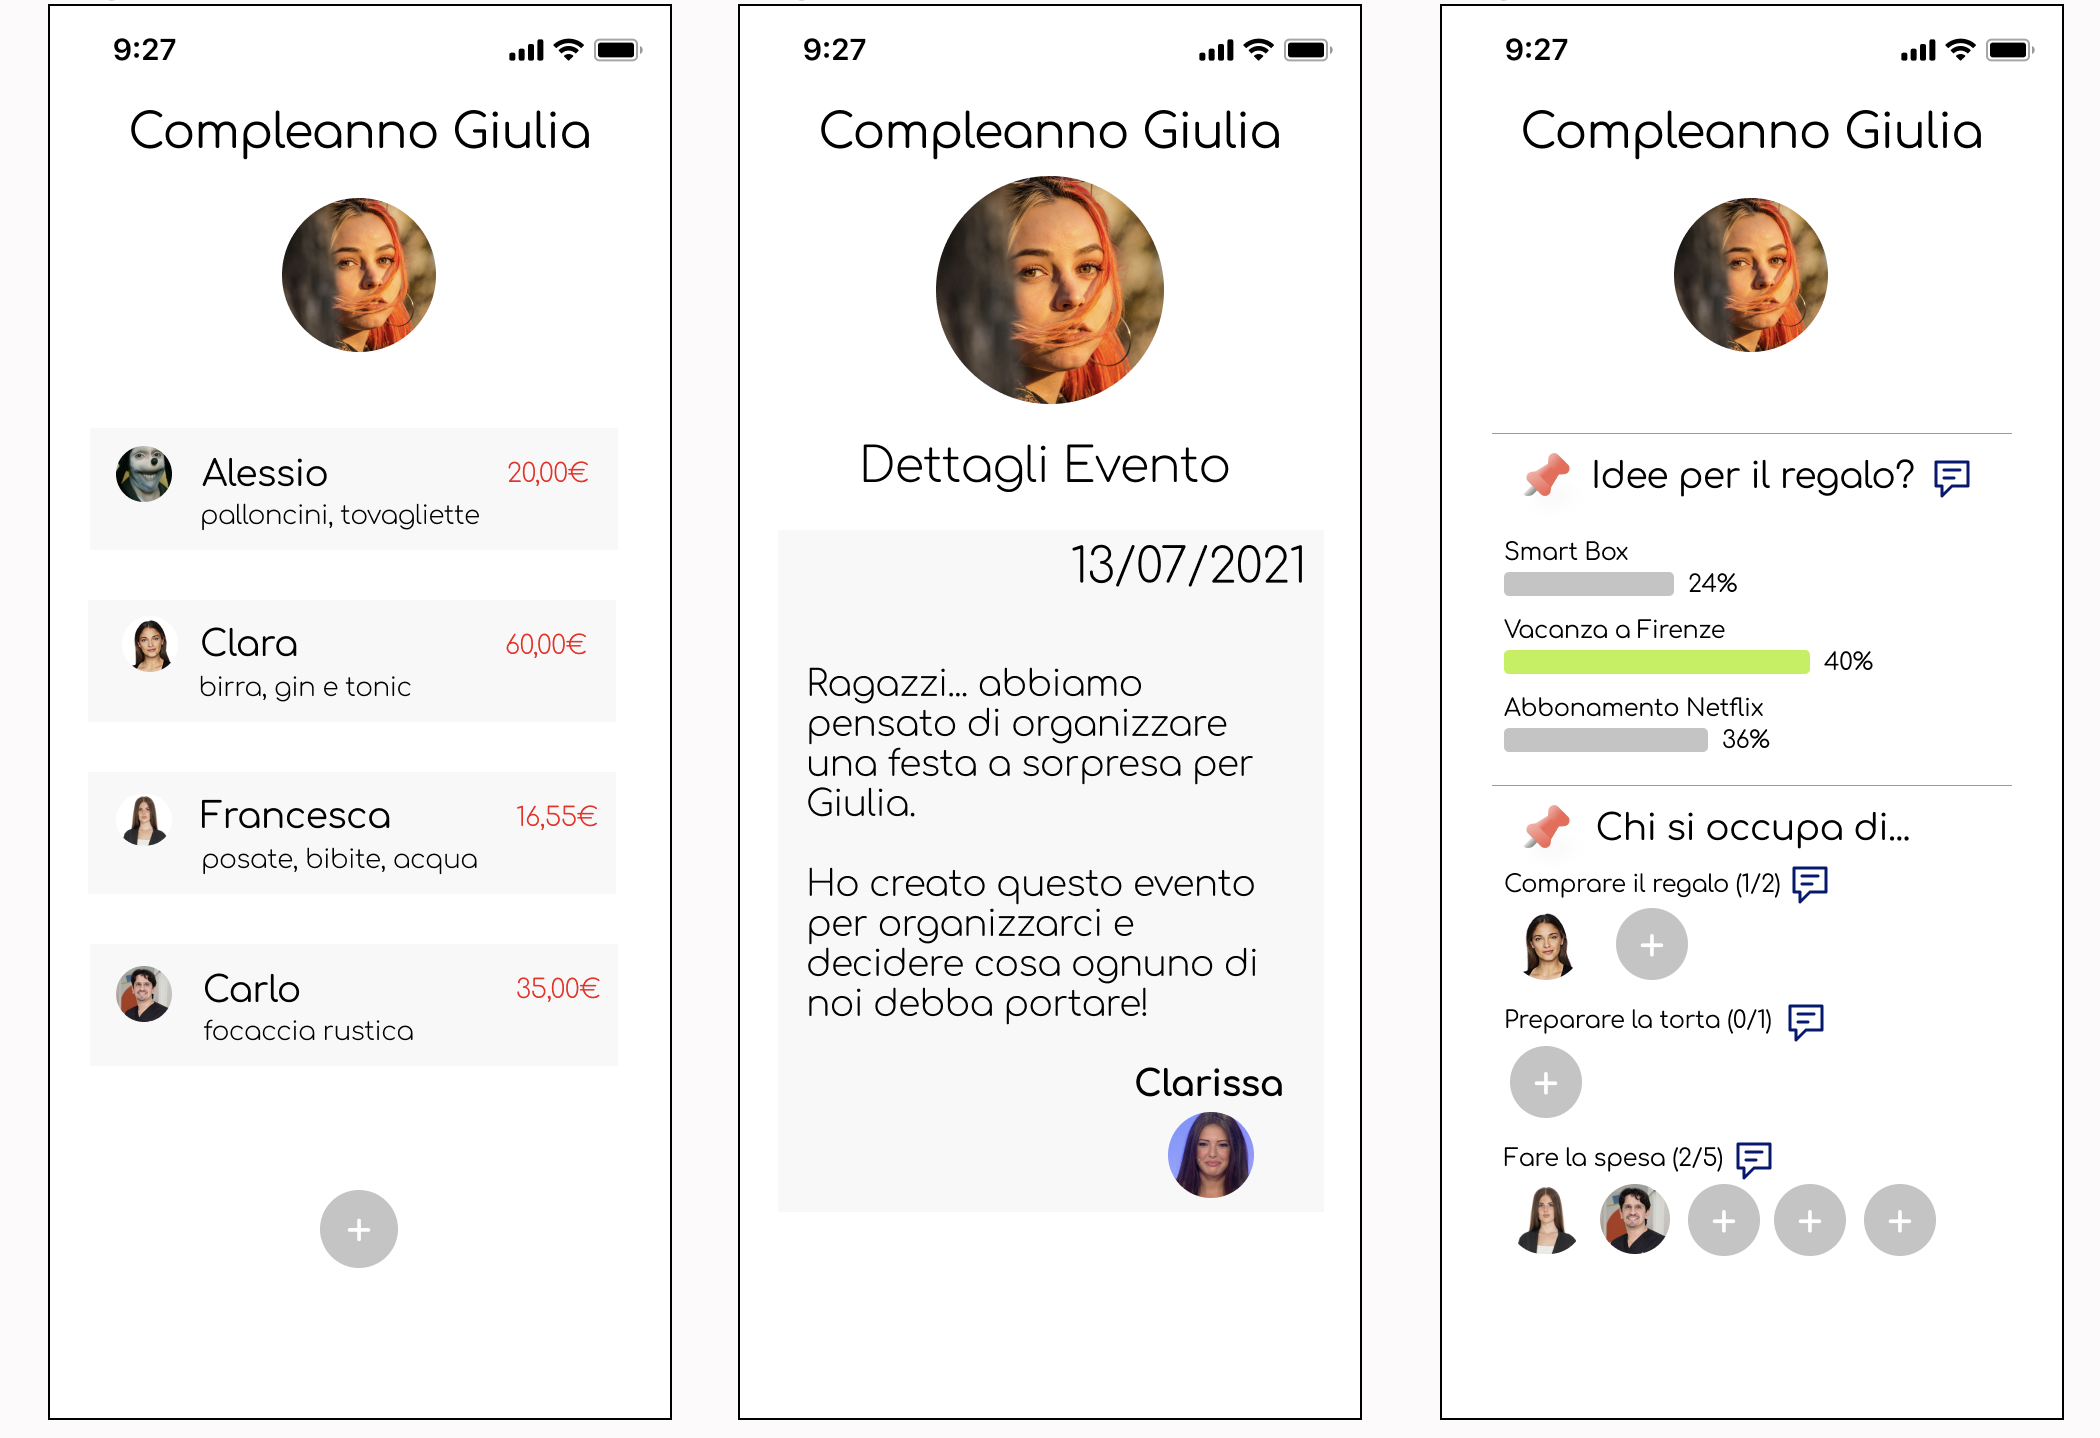
\includegraphics[width=.8\linewidth]{mock2.png}
%			\caption{Mockups (2/2)}
		\end{figure}
	\end{frame}

	\begin{frame}[plain]
		\begin{tikzpicture}[overlay, remember picture]
			\node[anchor=center] at (current page.center) {
				\begin{beamercolorbox}[center]{title}
					{\Huge Grazie per l'attenzione}\\
					\Large Domande?
			\end{beamercolorbox}};
		\end{tikzpicture}
	\end{frame}


\end{document}